% ----------------------------------------
% Chapter: Stand der Technik
% ----------------------------------------
\chapter{Stand der Technik}
\label{chap:stand_der_technik}

Ein geschmierter Reibungskontakt kann auf vier Elemente des tribologischen Systems nach Czichos\cite{czichos} reduziert werden:
\begin{itemize}
    \item Grundkörper
    \item Gegenkörper
    \item Zischenstoff
    \item Umgebungsmedium
\end{itemize}
% ----------------------------------------
% Fig: Das tribologische System
% ----------------------------------------
\begin{figure}[htb]
    \centering
    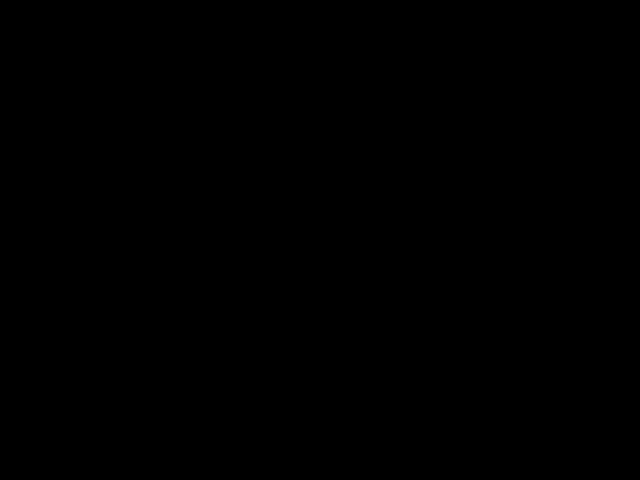
\includegraphics[width=5cm]{./images/blank_img.jpg}
    \caption{Das tribologische System}
    \label{fig:das_tribologische_system}
\end{figure}

Um ein besseres Verständnis der EHD-Schmierung zu haben, wird in diesem Abschnitt zuerst die Kennwerte des Zwischenstoffes (Schmiermittel) und der beiden Kontaktelementen (Grund- und Gegenkörper) ausführlich besprochen.
Danach wird der Mechanismus der EHD-Schmierung beleuchtet und am Ende wird die Arbeit von Hamrock und Dowson zur theoretischen Bestimmung der Schmierfilmdicke erwähnt.

% ----------------------------------------
% Sec: Eigenschaften des Schmiermittels
% ----------------------------------------
\section{Eigenschaften des Schmiermittels}
\label{sec:eigenschaften_des_schmiermittels}

\info[inline]{Viskosität}
Viskosität, die auch als innere Reibung bezeichnet wird, ist die wichtigste Kenngröße eines Schmierstoffes.
Sie beschreibt die Zähigkeit von Flüssigkeiten und Gasen.
Je größer die Viskosität ist, desto dickflüssiger ist das Fluid und je niedriger die Viskosität, desto dünnflüssiger ist es.
Ein Modell des Parallelplattenversuchs veranschaulicht das FließVerhalten des Schmierstoffes, Abbildung \ref{fig:geschwindigkeitsprofil_parallelplattenversuch}.
% ----------------------------------------
% Fig: Geschwindigkeitsprofil in einem Parallelplattenversuch
% ----------------------------------------
\begin{figure}[htb]
    \centering
    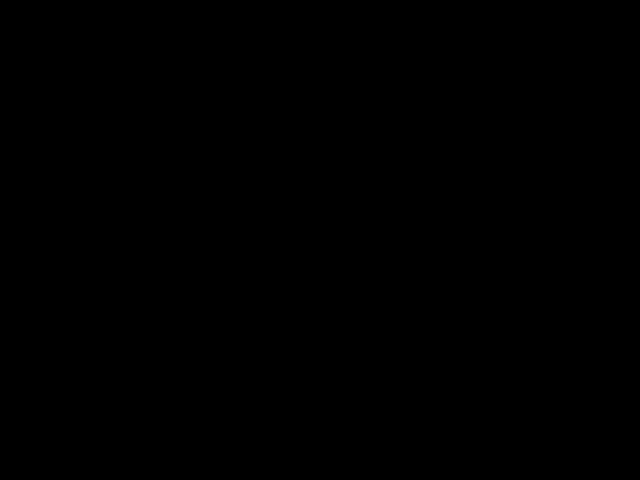
\includegraphics[width=5cm]{./images/blank_img.jpg}
    \caption{Geschwindigkeitsprofil in einem Parallelplattenversuch}
    \label{fig:geschwindigkeitsprofil_parallelplattenversuch}
\end{figure}

Für eine Newtonsche Flüssigkeit ist das Schergefälle $G = du/dz$ direkt proportional zur der Schubspannung $\tau$
% ----------------------------------------
% Eq: Schergefälle
% ----------------------------------------
\begin{equation}
    G = k \cdot \tau
    \label{eq:schergefaelle}
\end{equation}

Die dynamische Viskosität (oder Viskosität) ist das Verhältnis von Schubspannung und Geschwindigkeitsgradient und ist der Kehrwert der Fluidität $k$ im Newtonschen Schubspannungsgesetz (\ref{eq:schergefaelle}).
% ----------------------------------------
% Eq: Dynamische Viskosität
% ----------------------------------------
\begin{equation}
    \eta = \frac{1}{k} = \frac{\tau}{G} = \frac{\tau}{du/dz}
    \label{eq:dynamische_viskositaet}
\end{equation}

Die kinematische Viskosität ergibt sich aus der dynamischen Viskosität durch die Division mit der Dichte des Fluids.
% ----------------------------------------
% Eq: Dynamische Viskosität
% ----------------------------------------
\begin{equation}
    \nu = \frac{\eta}{\rho}
    \label{eq:kinematische_viskotitaet}
\end{equation}

Im Si-Einheitensystem hat die dynamische Viskosität als Einheit $N \cdot s/m^2$ oder $Pa \cdot s$ und die kinematische Viskosität als Einheit $m^2/s$.
Ein Stoff hat die Viskosität $1~N \cdot s/m^2$, wenn er in zwischen zwei Platten, die Größe von $1~m^2$ und einen Abstand von $1~m$ haben, befindet und man braucht $1~N$, um die zwei Platten gegeneinander mit einer Geschwindigkeit von $1~m/s$ zu verschieben.

\info[inline]{Temperatureffekt}
Die Temperatur hat eine große Effekt auf der Viskosität aller fließfähigen Stoffe.
Mit steigender Temperatur sinkt die Viskosität der Flüssigkeiten ab.
Diese Effekt kann experimentell mittel eines Viskosimeters und rechnerisch nach Cameron bestimmt werden.

Die einfachste Gleichung nach Reynold lautet:
% ----------------------------------------
% Eq: Dynamische Viskosität nach Reynold
% ----------------------------------------
\begin{equation}
    \eta = \eta_{s} \cdot exp (-\beta \cdot \Delta\phi)
    \label{eq:dynamische_viskositaet_reynold}
\end{equation}
%
wobei $\eta_{s}$ ist die Viskosität des Schmierstoffes bei der Temperatur $\phi_{s}$, $\eta$ ist die Viskosität des Schmierstoffes bei der Temperatur $\phi$, $\Delta{\phi}$ ist die Temperaturdifferenz ($\eta = \eta_{s} + \Delta{\phi}$) und $\beta$ ist die thermoviskose Konstante.\improvement{check the formel}
% ----------------------------------------
% Eq: Dynamische Viskosität nach Cameron
% ----------------------------------------
\begin{equation}
    \eta(\phi) = k_1 \cdot exp \left( \frac{k_2}{\phi + 95} \right)
    \label{eq:dynamische_viskositaet_cameron}
\end{equation}

\info[inline]{Viskositätsindex}
Die Temperaturabhängigkeit der kinematischen Viskosität eines Schmieröls wird auch von einem Viskositätsindex (VI oder KVI) beschreibt.
Der Viskositätsindex basiert auf einer Skalar, in der zwei unterschiedlichen Öltypen mit deutlich abweichenden Viskosität-Temperaturverhalten zugeordnet wurden.
Das Öl, das starke Veränderung der Viskosität ist, wird mit 0 oder LVI (low viscosity index) indiziert.
Das andere Öl wird mit 100 oder HVI (high viscosity index) gekennzeichnet.
Aus dem Vergleich der kinematischen Viskosität eines zu beschreibenden Öls mit diesen beiden Referenzölen bei $100^\circ$  ergibt sich dessen Viskositätsindex, Formel \ref{eq:viskositaetsindex}.
% ----------------------------------------
% Eq: Viskositätsindex
% ----------------------------------------
\begin{equation}
    VI (oder KVI) = \frac{\nu_0 - \nu}{\nu_0 - \nu_{100}}
    \label{eq:viskositaetsindex}
\end{equation}
%
In der VI-Definition ist es angenommen, dass die Veränderung der Viskosität mit Temperatur von drei Ölen linear ist.
Die Linearisierung ist nach Walther\cite{walther} und wird in der Abbildung~\ref{fig:variation_der_viskositaet_mit_temperatur} für das Mineralöle dargestellt.
% ----------------------------------------
% Fig: Naeherungsgleichung der Viskosität-Temperatur nach Walther
% ----------------------------------------
\begin{figure}[htb]
    \centering
    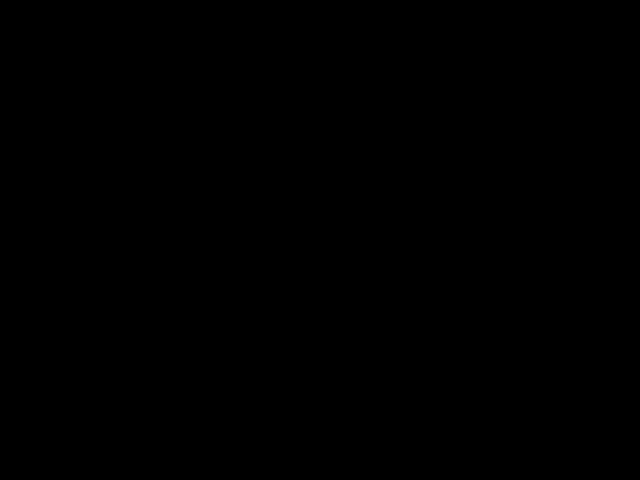
\includegraphics[width=5cm]{./images/blank_img.jpg}
    \caption{Variation der Viskosität mit Temperatur}
    \label{fig:variation_der_viskositaet_mit_temperatur}
\end{figure}

\info[inline]{Einfluss von Druck auf Viskosität}
Mit steigendem Druck nimmt die Viskosität aller Schmieröle zu.
% ----------------------------------------
% Fig: Viskosität - Druck - Verhalte
% ----------------------------------------
\begin{figure}[htb]
    \centering
    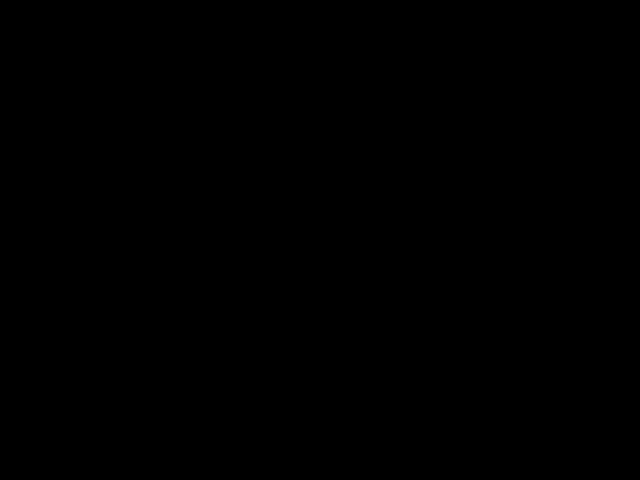
\includegraphics[width=5cm]{./images/blank_img.jpg}
    \caption{Dynamische Viskosität in Abhängigkeit vom Druck}
    \label{fig:dynamische_viskositaet_in_abhaengigkeit_vom_druck}
\end{figure}
%
Allerdings verändert sich das Schmiermittel unter dem für die EHD-Kontakte ernormen Druck schlagartig.
Die Viskosität nimt rapide zu und der Schmierstoff erreicht einem festen Zustand.
Nach Barus kann die Viskosität mit der unteren Formel berechnet werden
% ----------------------------------------
% Eq: Viskositätsindex
% ----------------------------------------
\begin{equation}
    \eta = \eta_0 \cdot exp(\alpha_p \cdot p)
    \label{eq:dynamische_viskositaet_druck_barus}
\end{equation}
%
wobei $\eta_0$ die Viskosität beim Atmosphärendruck und $\alpha_p$ der Druckkoeffizient der Viskosität ist.

Der Druckkoeffizient der Viskosität $\alpha_p$ ist nicht eine Konstante, sodern eine Funktion der Temperatur.
Diese Abhängigkeit wird in Abbildung~\ref{fig:druckkoeffizient_temperatur} für die Referenzöle der FVA gezeigt.
% ----------------------------------------
% Fig: Druckkoeffizient der FVA-Referenzöle in Abhängigkeit von der Temperatur
% ----------------------------------------
\begin{figure}[htb]
    \centering
    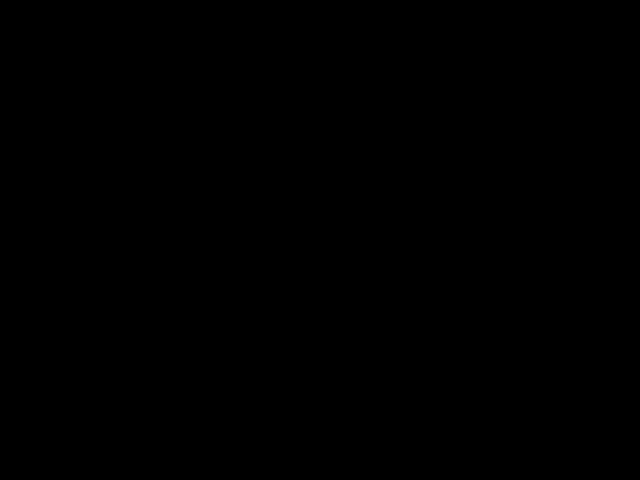
\includegraphics[width=5cm]{./images/blank_img.jpg}
    \caption{Verhalten des Druckkoeffizienten in Abhängigkeit von der Temperatur}
    \label{fig:druckkoeffizient_temperatur}
\end{figure}
%

\info[inline]{Dichte}
Für eine numerische Schmierfilmdickenmessung ist es notwendig zu wissen, wie die Dichte des Schmierstoffes unter verschiedenen Druck verhält.
Die Form des Schmierfilms kann nicht richtig berechnet werden, wenn diese Eigenschaft vernachlässigt wird.
Die Kompressibilität eines Schmierstoffes C ist nach Chu und Cameron mit folgender Fomel zu berechnen:
% ----------------------------------------
% Eq: Die Kompressibilität eines Schmierstoffes
% ----------------------------------------
\begin{equation}
    \label{eq:kompressibilitaet}
    C = \left( \frac{1}{\rho} \right) \frac{d\rho}{dp} = \left( \frac{1}{V} \right) \frac{dV}{dp}
\end{equation}
%
wobei V das Volumen und $dV$ die Änderungs des Volumens ist.

Die Dichte der Mineralöle ist nach Hirano\cite{hirano} mit folgender Formel zu berechnen
% ----------------------------------------
% Eq: Dichte nach Hirano
% ----------------------------------------
\begin{equation}
    \label{eq:dichte_hirano}
    \rho = \rho_0 \left( 1 + \frac{0,6p}{1 + 1,7p} \right)
\end{equation}
%
wobei $p$ in GPa und $\rho_0$ die Dichte beim normalen Luftdruck ($0,87 kg/m^3$ bei $20^\circ C$) ist.
% ----------------------------------------
% Fig: Druckkoeffizient der FVA-Referenzöle in Abhängigkeit von der Temperatur
% ----------------------------------------
\begin{figure}[htb]
    \centering
    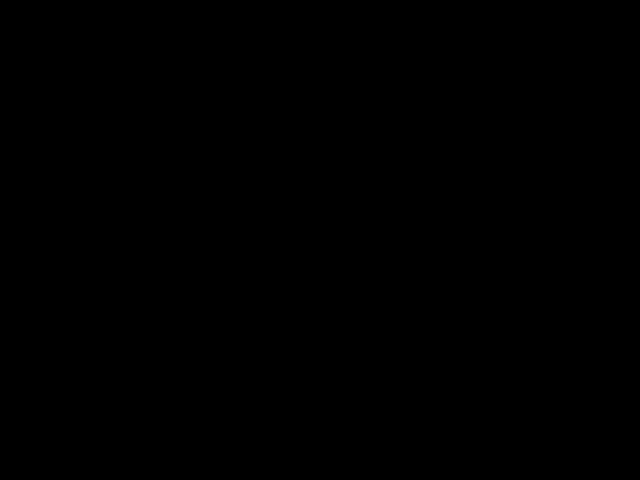
\includegraphics[width=5cm]{./images/blank_img.jpg}
    \caption{Variation der Dichte bei verschiedenen Drücke}
    \label{fig:variation_der_dichte_bei_verschiedenen_druecke}
\end{figure}

\info[inline]{Brechungsindex}
Für die Messverfahren, die auf optischen Interferometrie basieren, brauch man die Abhängigkeit zwischen der Dichte und dem Brechungsindex des Schmierstoffes.
Nach Gohar wird das Verhältnis mit der Formel\ref{eq:dichte_brechnungsindex} beschrieben.
% ----------------------------------------
% Eq: Dichte und Brechungsindex
% ----------------------------------------
\begin{equation}
    \label{eq:dichte_brechnungsindex}
    cp = \frac{n^2 - 1}{n^2 + 2}
\end{equation}
%
wobei $c$ ein Ölkonstante ist (zB: SAE30, c = 0,33).
Der Brechungsindex für meist Mineralöle bei normalen Luftdruck ist c.a 1,51.


\info[inline]{Wärmeleitfähigkeit}
Um die Temperaturerhöhung des Schmierstoffes unter Schubspannung zu schätzen, ist dessen Wärmeleitfähigkeit $k$ nötig.
Nach Cameron\cite{cameron} kann diese Größe beim normalen Luftdruck mit folgender Formel berechnet werden.
% ----------------------------------------
% Eq: Wärmeleitfähigkeit
% ----------------------------------------
\begin{equation}
    \label{eq:waermeleitfaehigkeit}
    k = \frac{0,1173 - 6,33 \times 10^{-5} \theta}{\rho_0}
\end{equation}
%
wobei $\theta$ die absolute Temperatur in $K$ und $\rho_0$ die Dichte in $kg/m^3$ ist.

\info[inline]{Verfestigung der Schmierung bei hohem Druck}

\info[inline]{Newtonsche Fluide}
Wenn die Viskosität eines Fluids von der Schubspannung abhängig ist, wird das Fluid als newtonsches Fluid bezeichnet.
Wenn diese Bedingung nicht mehr gilt, ist das Fluid nicht newtonsch.
Für die Bestimmung der Schmierfilmdicke werden alle Fluide in Rahmen dieser Arbeit als newtonsche Fluide angenommen.

% ----------------------------------------
% Sec: Betrachtung des EHD-Kontaktes
% ----------------------------------------
\section{Betrachtung des EHD-Kontaktes}
\label{sec:betrachtung_des_ehd_kontaktes}

\begin{itemize}
    \item Nichtkonformer Kontakt
    \item Hertzsche Gesetz
        \begin{itemize}
            \item Kugel-Kugel
            \item Kugel-Platte
        \end{itemize}
    \item Kontakt von beschichteten Körpern
\end{itemize}

% ----------------------------------------
% Sec: Elastohydrodynamische Schmiertheorie
% ----------------------------------------
\section{Elastohydrodynamische Schmiertheorie}
\label{elastohydrodynamische_schmiertheorie}

Erklärung, wie EHD funktioniert

% ----------------------------------------
% Sec: Schmierung nach Hamrock und Dowson
% ----------------------------------------
\section{Schmierfilmdicke nach Hamrock und Dowson}
\label{sec:schmierfilmdicke_nach_hamrock_und_dowson}
Erklärung, wie mann die Schmierfilmdicke berechnen kann
